\section{Supplementary Materials for Section~\ref{section:experiments}}
\label{section:supp-to-experiment}

Figures~\ref{fig:banditron-points},~\ref{fig:linearova-points}, and~\ref{fig:rationalova-points} show the final decision boundaries learned by each algorithm on the two datasets (Figures~\ref{figure:number-of-mistakes-strongly-separable-dataset} and~\ref{figure:number-of-mistakes-weakly-separable-dataset}), 
after $T = 5 \times 10^6$ rounds. We used the version of Banditron
with exploration rate of 0.02, which explores the most.

\begin{figure}[h!]
    \centering
    \begin{subfigure}[b]{0.25\textwidth}
        \captionsetup{justification=centering}
        \begin{center}
        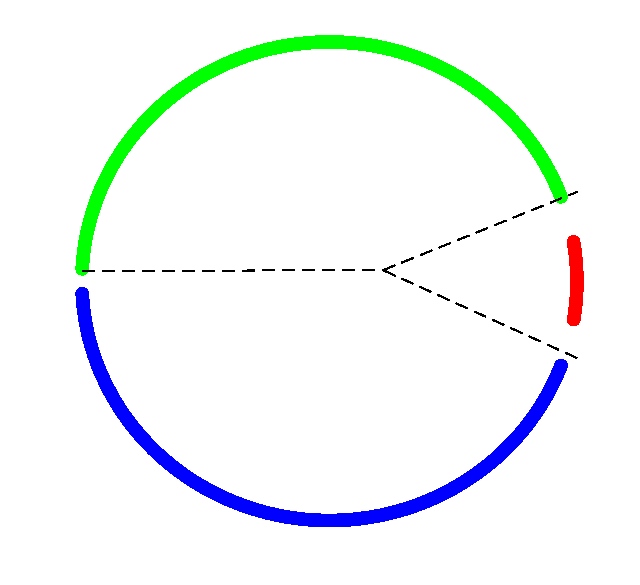
\includegraphics[width=\textwidth, trim={0, 0cm, 0, 0}, clip]{figures/strong_banditron_points}
        \caption{Strongly separable case}
        \end{center}
    \end{subfigure}
    \begin{subfigure}[b]{0.25\textwidth}
        \captionsetup{justification=centering}
        \centering
        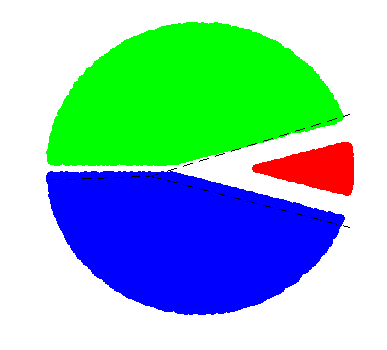
\includegraphics[width=\textwidth, trim={0, 0cm, 0, 0}, clip]{figures/weak_banditron_points}
         \caption{Weakly separable case}
    \end{subfigure}
    \captionsetup{justification=centering}
    \caption{\textsc{Banditron}'s final decision boundaries}
     \label{fig:banditron-points}
\end{figure}

\begin{figure}[h!]
    \centering
    \begin{subfigure}[b]{0.25\textwidth}
        \captionsetup{justification=centering}
        \begin{center}
        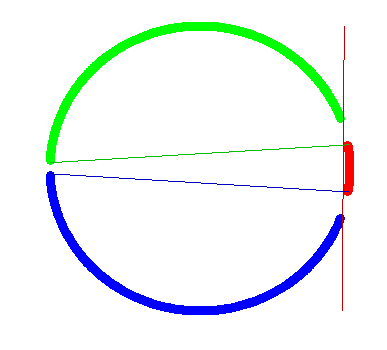
\includegraphics[width=\textwidth, trim={0, 0cm, 0, 0}, clip]{figures/strong_linear_ova_points}
        \caption{Strongly separable case}
        \end{center}
    \end{subfigure}
    \begin{subfigure}[b]{0.25\textwidth}
        \captionsetup{justification=centering}
        \centering
        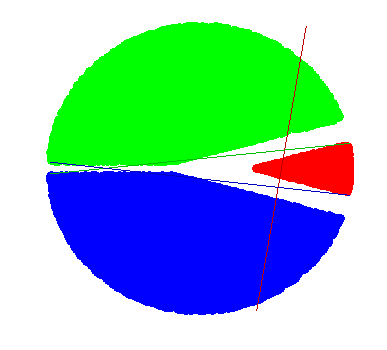
\includegraphics[width=\textwidth, trim={0, 0cm, 0, 0}, clip]{figures/weak_linear_ova_points}
         \caption{Weakly separable case}
    \end{subfigure}
    \captionsetup{justification=centering}
    \caption{Algorithm~\ref{algorithm:algorithm-for-strongly-linearly-separable-examples}'s final decision boundaries}
    \label{fig:linearova-points}
\end{figure}
%Our Algorithm with linear kernel (
%To better understand how each algorithm works,
%Our Algorithm with rational kernel (

\begin{figure}[h!]
    \centering
    \begin{subfigure}[b]{0.25\textwidth}
        \captionsetup{justification=centering}
        \begin{center}
        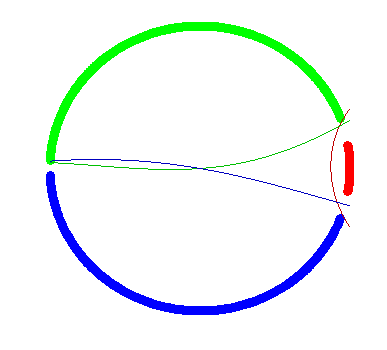
\includegraphics[width=\textwidth, trim={0, 0cm, 0, 0}, clip]{figures/strong_rational_ova_points}
        \caption{Strongly separable case}
        \end{center}
    \end{subfigure}
    \begin{subfigure}[b]{0.25\textwidth}
        \captionsetup{justification=centering}
        \centering
        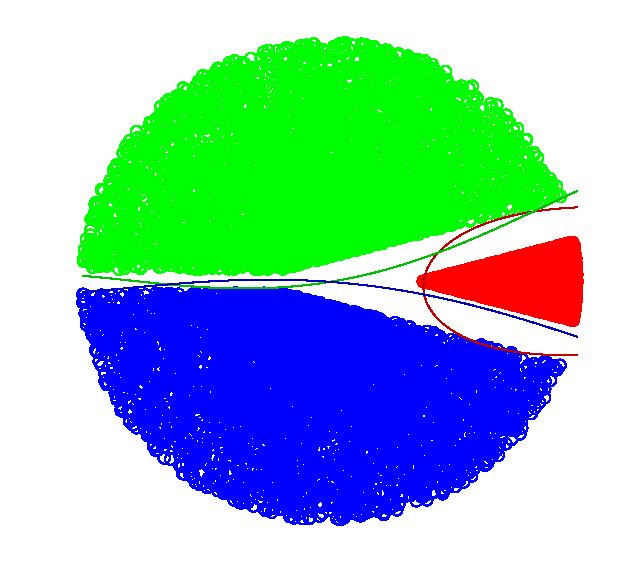
\includegraphics[width=\textwidth, trim={0, 0cm, 0, 0}, clip]{figures/weak_rational_ova_points}
         \caption{Weakly separable case}
    \end{subfigure}
    \captionsetup{justification=centering}
    \caption{Algorithm~\ref{algorithm:kernelized} (with rational kernel)'s final decision boundaries}
    \label{fig:rationalova-points}
\end{figure}
